\section{Designkonzept}

% Klassenzimmer --> Flugschule um weiteren Komponenten sinnvoll einzufügen
%--> erstellung eines händischen drahtmodells -->
% --> Definition der einzelnen Komponenten --> Maaße definieren
% --> Visio Zeichnung 
% --> Interaktionen definieren
% Flugsimulator als erweiterung

%TODO Mention Phong from Flightsimulator

Als grundlegende Idee wurde zunächst ein Vorlesungsaal vorgeschlagen.
Um weitere Komponenten aus den Anforderungen an diese Arbeit sinnvoll umzusetzen,
wurde die grundlegende Idee überdacht und neu definiert als Klassenzimmer einer Flugschule.
\newparagraph
Um eine erste Vorstellung des Klassenzimmers zu bekommen wurde zunächst eine händische Zeichnung angefertigt.
Diese ist in der Abbildung \ref{fig:KlassenzimmerSkizze} dargestellt.
\begin{figure}[H]
  \centering
  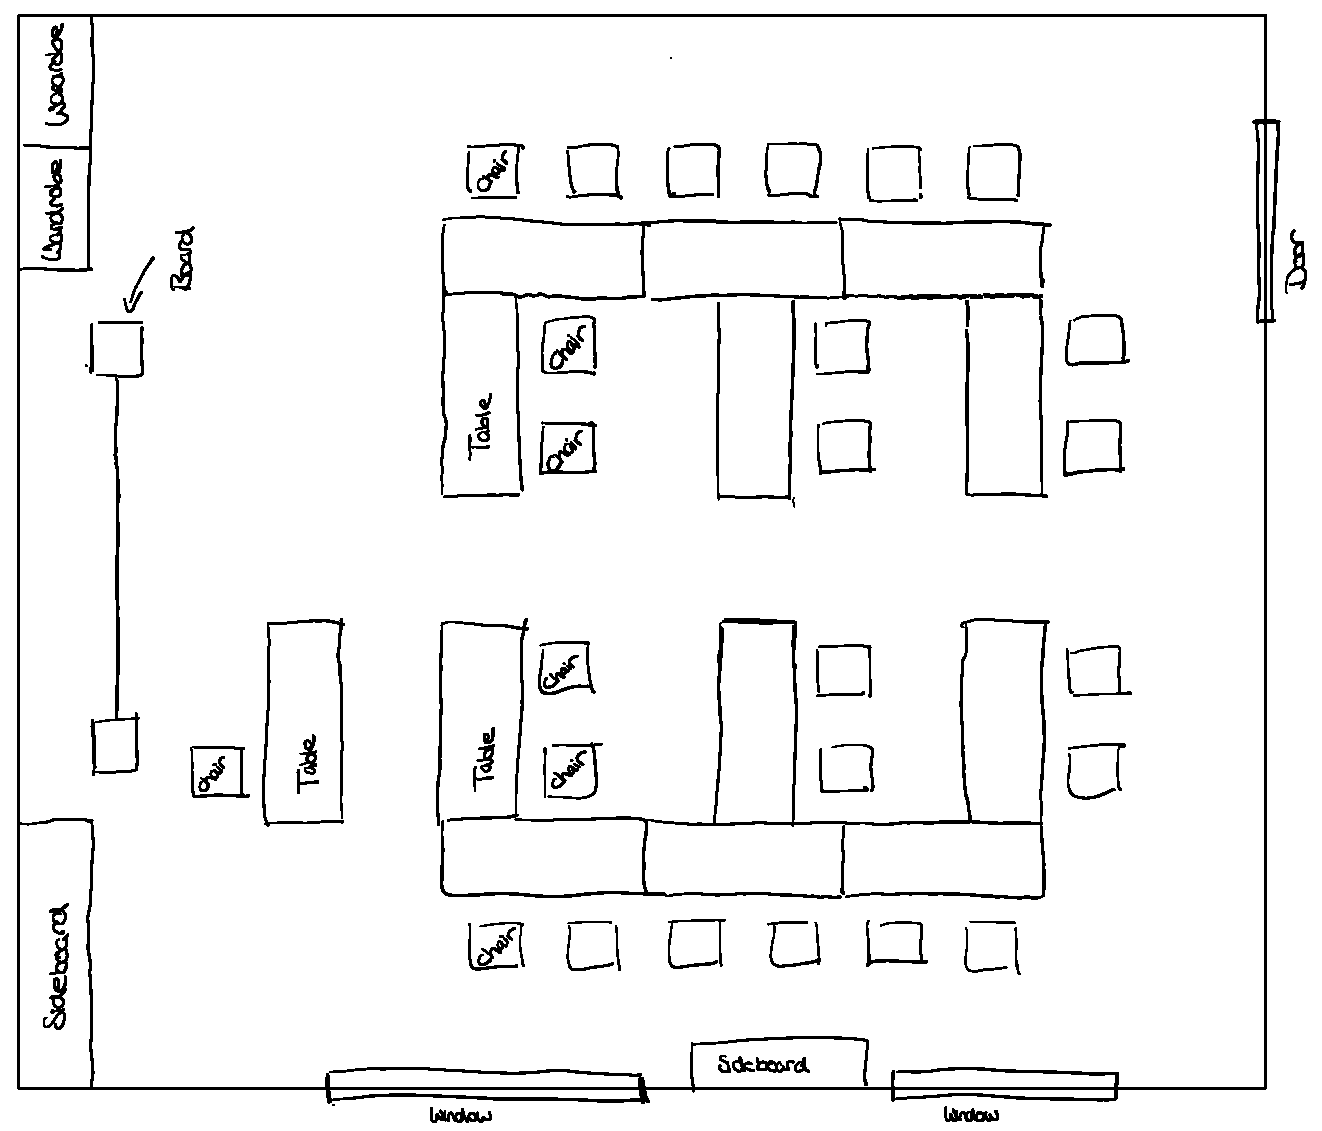
\includegraphics[width=1\textwidth]{images/roomModel_OneNote.pdf}
  \caption{Klassenzimmer Skizze}
  \label{fig:KlassenzimmerSkizze}
\end{figure}\noindent
Anschließend wurde der Raum maßstabsgetreu in einem Bauplan gezeichnet um so die Abstände und Maaße teilweise zu definieren.
Diese Zeichnung ist in der Abbildung \ref{fig:KlassenzimmerEntwurf} dargestellt.

\begin{figure}[H]
  \centering
  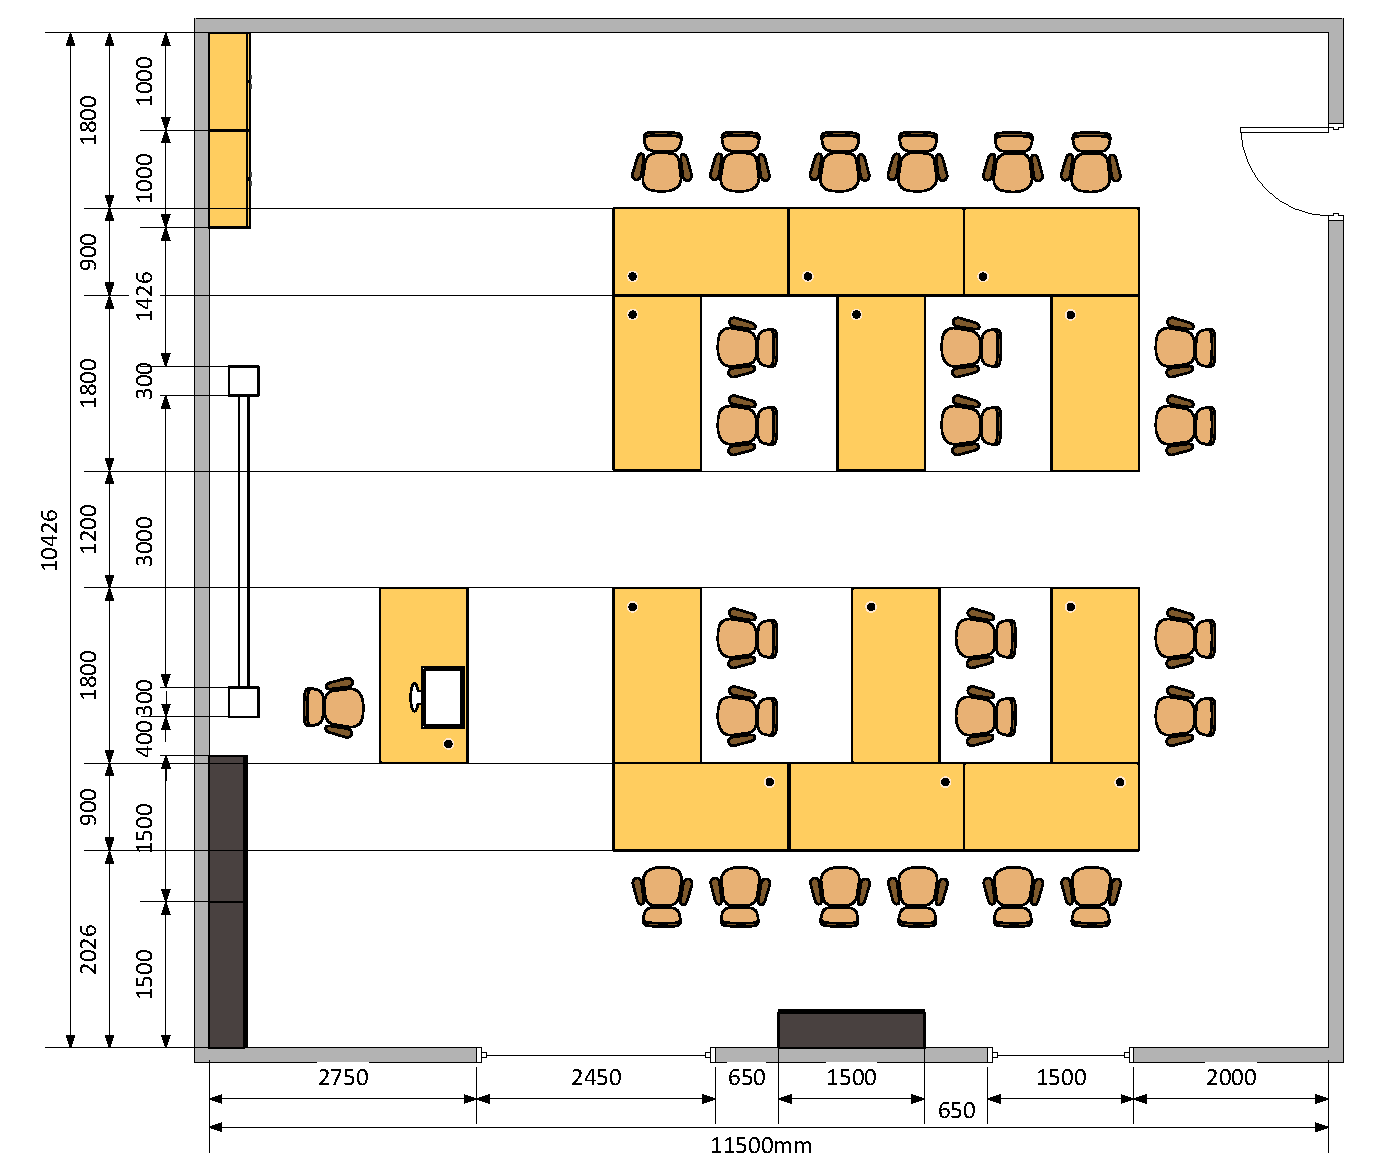
\includegraphics[width=1\textwidth]{images/roomModelVisio.pdf}
  \caption{Klassenzimmer Entwurf mit Bemaßung}
  \label{fig:KlassenzimmerEntwurf}
\end{figure}\noindent